\documentclass[10pt]{article}

\def\Type{LessonCaelan}
\def\TypeNum{Lesson 11}
\def\TypeTitle{Local Extrema and the First Derivative Test }
\def\Semester{Fall 2021} %Not Used 
\def\Course{MATH 1190 \& 1210}
\def\Targets{ {\bf \color{ForestGreen}D2} , {\bf \color{ForestGreen}D3} }

\usepackage{preambleDJ}
\usepackage{enumerate}

%%%%%%%%%%%% BEGIN DOCUMENT %%%%%%%%%%%%%%%
%%%%%%%%%%%% BEGIN DOCUMENT %%%%%%%%%%%%%%%
%%%%%%%%%%%% BEGIN DOCUMENT %%%%%%%%%%%%%%%
%%%%%%%%%%%% BEGIN DOCUMENT %%%%%%%%%%%%%%%
%%%%%%%%%%%% BEGIN DOCUMENT %%%%%%%%%%%%%%%

%%%%%%%%%%%% BEGIN DOCUMENT %%%%%%%%%%%%%%%
%%%%%%%%%%%% BEGIN DOCUMENT %%%%%%%%%%%%%%%
%%%%%%%%%%%% BEGIN DOCUMENT %%%%%%%%%%%%%%%
%%%%%%%%%%%% BEGIN DOCUMENT %%%%%%%%%%%%%%%
%%%%%%%%%%%% BEGIN DOCUMENT %%%%%%%%%%%%%%%

\begin{document}

\pagestyle{otherpages}
\thispagestyle{firstpage}
\vs{.6}

\textbf{Intended Learning Outcomes}
After this lesson, you will be able to 

\begin{itemize}
    \item Identify increasing/decreasing intervals and critical numbers of a function from given graph or formula. (\target{A1})
    \item Represent concepts such as derivatives, local extrema, and critical number graphically. (\target{A1})
    \item Apply the First Derivative Test to determine the local extrema of a function graphically and algebraically. (\target{A2})
\end{itemize}

\vspace{-0.5cm}

\hrulefill\\

In this activity, we establish a means of finding local extreme values (also called relative extreme values) of a function using properties of the derivative. First, review some key ideas from the online pre-class activity to prepare yourself for the important ideas of the lesson.\\

{\bf \textcolor{blue}{Warm-up exercise 1.}}  Fill in the blanks to complete the definition of a critical number, then respond to the prompt below.
%
 \important{Definition: Critical Number}
    {
    A {\bf critical number} of a function $f$ is a number $c$ at which $f$ is \rule[-8pt]{1.5in}{0.4pt} and either
    \begin{center}
    $f'(c) = \rule[-8pt]{0.5in}{0.4pt}$ \quad\quad\quad or \quad\quad\quad $f'(c)$ \rule[-8pt]{2in}{0.4pt}.
    \end{center}
    }
    
    {\bf TRUE or FALSE?} $\displaystyle f(x)=\frac1x$ has exactly 1 critical number. \hfill (circle one): \hfill {\bf TRUE} \hfill {\bf FALSE}
    
    \vfill

{\bf \textcolor{blue}{Warm-up exercise 2.}} Fill in the blanks to complete the statement of the First Derivative Test as it appeared in the online pre-class activity.

\begin{minipage}[t][2.75in][t]{0.65\textwidth}
 \important{First Derivative Test}
{
Suppose that $c$ is a \rule[-8pt]{2in}{0.4pt} of a continuous function $f$.
\begin{enumerate}[(a)]
\item If $f'$ changes from \rule[-8pt]{0.5in}{0.4pt} to \rule[-8pt]{0.5in}{0.4pt} at $c$, then $f$ has a local maximum at $c$.
\item If $f'$ changes from \rule[-8pt]{0.5in}{0.4pt} to \rule[-8pt]{0.5in}{0.4pt} at $c$, then $f$ has a local minimum at $c$.
\item If $f'$ does not change sign at $c$, then $f$ has \rule[-8pt]{1.25in}{0.4pt}\\[0.1in] \rule[-8pt]{3in}{0.4pt} at $c$.
\end{enumerate}
}
\end{minipage}
%
\hfill
%
\begin{minipage}[t][2.75in][t]{0.33\textwidth}
\,\\[-0.1in]

\includegraphics[width=0.95\textwidth]{images/1st derivative test.PNG}
\end{minipage}

\
 
\begin{minipage}[t]{0.6\textwidth}
{\bf \textcolor{blue}{Warm-up}}\exercise{\color{RedOrange}A1} Sketch the graph of a function $f$ satisfying the following:\\
 \begin{itemize}
 \item $f'(2)=0$ and $f(2)$ is a local/relative minimum
 \item $f'(4)=0$ and $f(4)$ is neither a maximum nor a minimum
 \item $f'(6)$ DNE and $f(6)$ is a local/relative maximum
 \end{itemize}
 \end{minipage}
 \hfill
 \begin{minipage}[t]{0.38\textwidth}
 \vspace{-0.2in}
 \begin{center}
	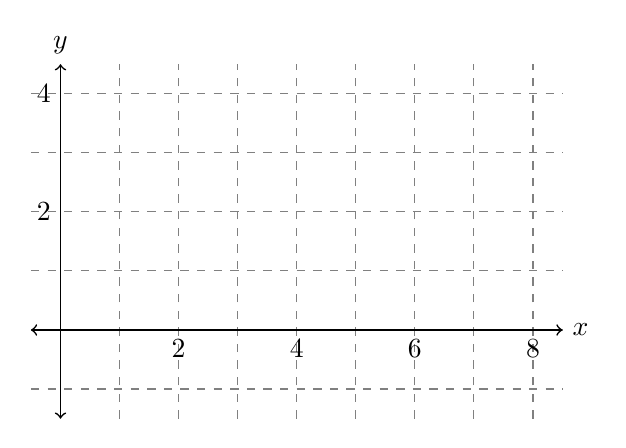
\begin{tikzpicture}[yscale=0.75,xscale=0.75]
	\draw[thin,color=gray,step=1,dashed] (-0.5,-1.5) grid (8.5,4.5); 
	\draw[semithick, <->] (-0.5,0)--(8.5,0) node[right]{$x$};   % x-axis
	\draw[semithick, <->] (0,-1.5)--(0,4.5) node[above]{$y$}; % y-axis
	\draw (2,0) node[below]{$2$};
	\draw (4,0) node[below]{$4$};
	\draw (6,0) node[below]{$6$};
	\draw (8,0) node[below]{$8$};
	\draw (0,2) node[left]{$2$};
	\draw (0,4) node[left]{$4$};
	\end{tikzpicture}
 \end{center}
 \end{minipage}

 %\end{document} %end here for written pre-class

 %%%%%%%%%%%%%
	%\newpage%%
 %%%%%%%%%%%%%

{\example{\color{RedOrange}A1,A2}} Let $g(x)=x-\ln(x^2+1)$.
%
\begin{enumerate}[(a)]
\item Find the critical numbers of $g$.

\vfill

\item Find the intervals where $g$ is increasing or decreasing.

\vfill
\vfill

\item At which critical number(s) does $g$ attain a local extreme value(s)? Explicitly cite a relevant test in your response.

\vfill

\end{enumerate}

\newpage

{\exercise{\color{RedOrange}A1,A2}} Let $f(x)=\dfrac{x}{x^2+1}$.
\begin{enumerate}
\item[(a)]Find the intervals where $f$ is increasing or decreasing. Draw a sign line to depict your answer, and record your final answer using interval notation. \\

\vfill
\vfill
\vfill


\item[(b)]Find the local maximum \& local minimum points of $f$. Explicitly cite a relevant test in your response. \\

\vfill
\vfill

\end{enumerate}

\newpage

\paragraph*{Note:} The next problem will test your conceptual understanding of what it means for a function to increase or decrease, as well as of the definition of a critical number. A variation of this problem appeared on an exam during the Fall 2023 semester.\\

\begin{minipage}{0.55\textwidth}
\exercise{\color{RedOrange}A1}  What would the critical numbers of the function $f$ be if...
\begin{enumerate}
\item[(a)] the curve pictured to the right is the graph of $f$?
\item[(b)] the curve pictured to the right is the graph of $f'$?
\end{enumerate}
On which intervals would the function $f$ be {\it decreasing} if...
\begin{enumerate}
\item[(c)] the curve pictured to the right is the graph of $f$?
\item[(d)] the curve pictured to the right is the graph of $f'$?
\end{enumerate}
\end{minipage}
%
\begin{minipage}{0.45\textwidth}
\begin{center}
    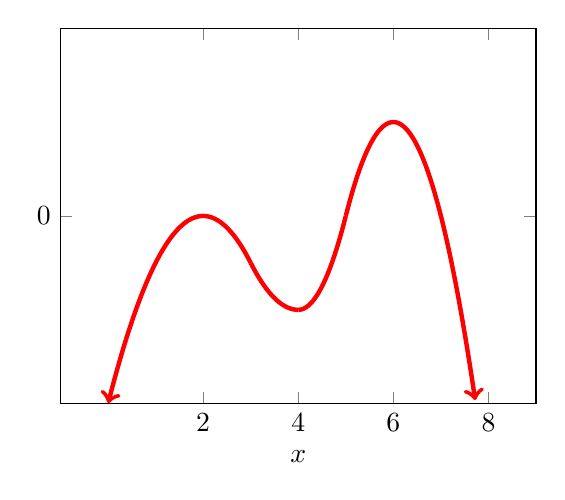
\begin{tikzpicture}[scale=1]
          \begin{axis}[
            xlabel={$x$},
            %grid = major,
            xtick       = {2,4,6,8},
            xticklabels = {$2$,$4$,$6$,$8$},
            ytick       = {0},
            yticklabels = {$0$},
            samples     = 320,
            domain      = -1:9,
            restrict y to domain=-4:4,
            xmin = -1, xmax = 9,
            ymin = -4, ymax = 4,
            height=2.5in, width=3in
          ]
          % old version of the curve
          %
          %\addplot[domain=-1:9, purple, ultra thick, mark=none] {-1/10*(x-1)*(x-4)^2*(x-7)};
          %
          %new version of the curve in pieces
          %
          \addplot[domain=-1:3, ultra thick, red,<-] {-(x-2)^2};
          \addplot[domain=3:4, ultra thick, red] {(x-4)^2-2};
          \addplot[domain=4:5, ultra thick, red] {2*(x-4)^2-2};
          \addplot[domain=5:9, ultra thick, red,->] {-2*(x-6)^2+2};
          %
        \end{axis}
    \end{tikzpicture}
\end{center}
\end{minipage}\\

\vspace{0.1in}

\,\hfill
\fbox{
    \begin{minipage}{ 0.18\textwidth}
    {\bf ANSWER (a):}
        \vspace{0.5in}
    \end{minipage}
    }
\hfill
    \fbox{
    \begin{minipage}{ 0.18\textwidth}
    {\bf ANSWER (b):}
        \vspace{0.5in}
    \end{minipage}
    }
\hfill
\fbox{
    \begin{minipage}{ 0.18\textwidth}
    {\bf ANSWER (c):}
        \vspace{0.5in}
    \end{minipage}
    }
\hfill
    \fbox{
    \begin{minipage}{ 0.18\textwidth}
    {\bf ANSWER (d):}
        \vspace{0.5in}
    \end{minipage}
    }
\hfill\,\\

Space is provided below for you to explain your answers.

\vfill


\paragraph*{Note:} The next problem will test your comprehension of warm-up exercise 1 and the Chain Rule.\\

{\bf\color{blue} Extra Practice 1.} \reversemarginpar\marginnote{\fbox{\bf\color{RedOrange} A2}} Find all critical numbers of $f(x)=\sqrt[3]{x^2-4x}$.

\vfill



\newpage

\paragraph*{Note:} The next 2 exercises make use of all the information in this worksheet and the associated pre-class activity. The goal is for you to continue to fluently apply the definition of a critical number, to find \& interpret the sign of the first derivative as it relates to whether a function is increasing or decreasing, and to use the First Derivative Test to classify critical numbers.\\

{\bf\color{blue} Extra Practice 2.} \reversemarginpar\marginnote{\fbox{\bf\color{RedOrange} A1, A2}} Let $f(x)=\ln(x^2-2x+1)$. 
\begin{enumerate}[(a)]
\item Find all critical numbers of $f$.
    \vfill
    
\item Find the intervals on which $f$ is increasing \& the intervals on which $f$ is decreasing.
    \vfill
    \vfill

\item At which $x$-values does $f$ have local maximum values? At which $x$-values does $f$ have local minimum values? Explain.
    \vfill
\end{enumerate}

%%%%%%%%%
\newpage%
%%%%%%%%%

{\bf\color{blue} Extra Practice 3.} \reversemarginpar\marginnote{\fbox{\bf\color{RedOrange} A1, A2}}

Let $f(x)=\dfrac15x^5-\dfrac53x^3+4x$.
\begin{enumerate}[(a)]
\item Find the critical numbers of $f$.
    \vfill
\item Find the intervals where $f$ is increasing or decreasing.
    \vfill
    \vfill
\item At which critical number(s) does $f$ attain local extrema? Explain.
    \vfill
    \vfill
\end{enumerate}

\end{document}


%%%%%%%%%%%%%%%%%%%%%%%%%%%%%%%%%%%%%%%%%%

%%%%%%%%%%%%%%%%

%%%%%%%%%%

%%%%% UNUSED EXERCISES %%%%%%

%%%%%%%

%%%%%%%%%%%%%%%%%%%%%%

%%%%%%%%%%%%%%%%%%%%%%%%%%%%%%%%%

{\example} Let $g(x)=x^{2/3}(x+2)$. You may take for granted that $g'(x)=\dfrac{5x+4}{3\sqrt[3]{x}}$. \\


(a) Find the critical numbers of $g$.

\vfill

(b) Find the intervals where $g$ is increasing or decreasing.

\vfill

(c) At which critical numbers does $g$ attain local maxima and minima? Explicitly cite a relevant test in your response.

\vfill


%(d) Find the intervals where the graph of $g$ is concave up and concave down.
%\vfill



%(e) Specify the $x$-coordinates of any points of inflection on the graph of $f$.
%\vfill


\,\hfill{\it Group Problem Solving}\hfill\,

{\exercise} Determine whether the following statement is {\bf TRUE} or {\bf FALSE}, and rigorously explain why.
\begin{center}
{\it
If  $f'$ is increasing on $(0, 5)$ and $f'(3) = 0$, then $f$ has a local minimum at $3$.
}
\end{center}

\vfill

{\bf\color{blue} Exam Practice 4.} Determine whether the following statement is {\bf TRUE} or {\bf FALSE}. Justify your answer mathematically using the first derivative.
\begin{center}
{\it
If $f'$ is increasing on $(0, 5)$ and $f'(3) = 0$, then $f$ has a local minimum at $3$.
}
\end{center}
    \vfill
